\section{Evaluation}
\label{sec:evaluation}
In this section we will provide an  evaluation for our introduced approaches based on the following research questions:
 \begin{description}
 	\item[Q1:] How do different event logs characteristics influence the performance of the secure multi-party computation?
 %	\item How does the number of chunks influence the performance of the secure multi-party computation?
 \item[Q2:] Does the proposed approach scale up with increasing the number of parallel chunks and what would be the effect of scalability on both the execution time and communication overhead between the computing parties?
\end{description}


\subsection{Datasets}
\label{sec:data}
To evaluate our approaches we run the experiment using the following real-world event logs:
\begin{description}
	\item[BPIC 2017] This event log captures the loan application process from a dutch financial institute. This event logs contains traces with a medium length, but is the largest investigated log in terms of number of events.
	\item[Traffic Fines] This event logs captures a process to handle the collection of fines from traffic law violations from a local police from Italy. It consists of rather short traces with a small number of different activities.
	%\item[Hospital Log] This event log captures treatments in a dutch hospital. The event log contains of long traces with an average of over 100 events in one trace.
		\item[Credit Requirement] This event log captures credit requirement process information in a dutch bank. The event log contains of short traces with only 8 unique events.
\end{description}
All of the introduced event logs capture a process from a single organization and not a cross-organizational business process. We decided to do so, because the existing public synthetic event logs\cite{borkowski2017event} for cross-organizational business processes consist only of a marginal number of events. Therefore, we have chosen event logs that contain a large number of cases and vary in the length of the traces, see table~\ref{tab:event_logs}. For the BPIC 2017, the data took about 5 hours till time out, we decide to selected 1000 traces randomly from the event log so we the log file could converge in a reasonable file.

To simulate  a cross-organizational setting we use Round Robin approach to assign each activity of each event log  to one party, assuming the business process is executed in a two party setting. We distribute the activities equally between both parties, so that each party executed half of the activity types for each log.

\begin{table}[!ht]
	
	\begin{tabularx}{\textwidth}{ X X X X X X}\\
		\toprule
		Event Log &No. of events &No. of cases & Avg. No. of events in case &Max No. of events in case & Min No. of events in case \\
		\midrule
		BPIC 2017 &		1,202,267 &	 31,509 & 38.16& 180 & 10\\
		Traffic Fines &	 561,470 & 	150,370 & 3.73& 20 & 2\\
		Hospital Log &	 150,291 &	 1,143 & 131.488 & 1814 & 1\\
		\bottomrule
	\end{tabularx}
	\caption{Event Logs for Evaluation}
	\label{tab:event_logs}
\end{table}

\subsection{Experimental Setup}
\label{sec:exp_setup}
To answer the above questions, we benchmark the performance of the proposed approach. We consider latency, throughput and the communication overhead as performance measures. 

\textbf{Latency.} We define latency as the amount of time needed to transform the 2 parties' event log securely into a DFG matrix. We report both the total execution time and the execution time of the chunk based sort. That would help to study how would help to study how the implementation of the proposed approach would be in a map/reduce like scheme. In subsection~\ref{sec:results}, the experiments show that changing the number of parallel chunks affects the chunk based sort only but the rest of the pipeline has a fixed execution time for the same dataset.

\textbf{Throughput.} We define throughput as the number of events that the system can process in a given amount of time. In our experiment, we report the number of events per minute as a measure of throughput.

\textbf{Communication Overhead.} In multi-party computation, the computing parties are communicating together so they can compute the final results securely. We define the communication overhead as the amount of data sent and received between the computing parties during the execution overhead. We report the values for each server. The communication overhead metric gives insights for how the system  would react in case the computing parties are remotely installed.

In the above performance measures, we perform the experiments until we have the DFG matrix, because it is the most sophisticated and time consuming portion of the pipeline, as it requires communicating both parties to build the matrix. Furthermore, once we have the DFG in secret shares, we can calculate the required queries in short time.

We provide the source code of our implementation on \emph{Github}\footnote{\url{https://github.com/Elkoumy/SecureMPCBPM}}. To implement our approaches we used the SecreC programming language from Cybernetica. Our implementation is run on the multi-party computation platform Sharemind\footnote{\url{https://sharemind-sdk.github.io}}.

To evaluate the performance of an approach we report the average maximum values for latency and the average value for both throughput the communication overhead. To calculate the mean execution time we run each experimental setting over 5 times and calculate the maximum execution time of the three servers. We used \emph{Nethogs}\footnote{\url{https://github.com/raboof/nethogs}} to measure the communication overhead and we report the average value per server.


\textbf{Hardware.} We run our experiments in a setting with three symmetrical servers as computation parties. These physical servers are connected through a local network. All of them use the same Sharemind setup. Each server has AMD Processor 6276 and 192 GB RAM and all the servers are connected using 1 gigabit Ethernet switch.


\subsection{Results}
\label{sec:results}


\begin{figure}[!htb]
	\centering
	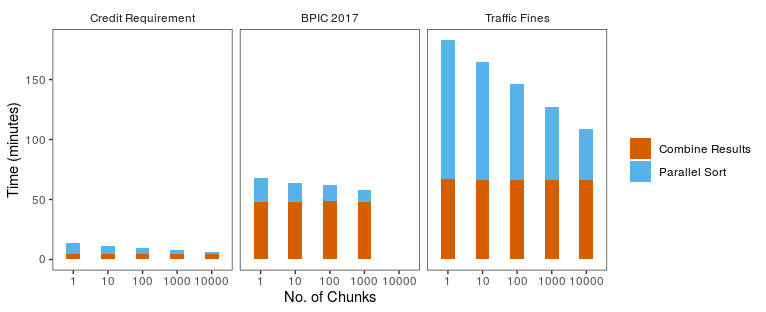
\includegraphics[width=.95\columnwidth]{figures/latency.png}
	\caption{Latency Benchmark: Execution Time vs no. of Chunks.}
	\label{fig:latency}
\end{figure}

\textbf{Latency Benchmark.} In fig~\ref{fig:latency}, we show the execution time to calculate the DFG matrix securely with different number of parallel chunks. We plot a bar for each chunk size. We split each bar to present the execution time of parallel sort in blue and the rest of the execution time in orange. From fig~\ref{fig:latency}, we can see that the execution time decreases with increasing the number of parallel chunks due to the execution of sort in parallel for each chunk separately. Because the sort complexity is $O(n log n)$, and after dividing data into chunks, the sorting complexity per chunk is $O((n/c) \: log  \: (n/c))$ where c is the number of parallel chunks. The execution time when using a single chunk, the sort is slower as c equals 1 and by increasing the number of chunks the factor $n/c$ decreases which reduces the execution time.  Furthermore, from fig~\ref{fig:latency}, we can observe that the execution time of the parallel sort, the blue part of the bars, changes with changing the number of parallel chunks and the combine results is almost fixed for each dataset. 

An interesting observation is that, both Credit Requirement and Traffic Fines datasets as the same number of events, and different number of unique events. The number of unique events increases the number of bits used to represent the event in the binary representation for the outer product step. Increasing the number of unique events per log makes the result matrix bigger which adds computation overhead. The same thing could be observed with the BPIC 2017 dataset as it has larger number of unique events.


\begin{figure}[!htb]
	\centering
	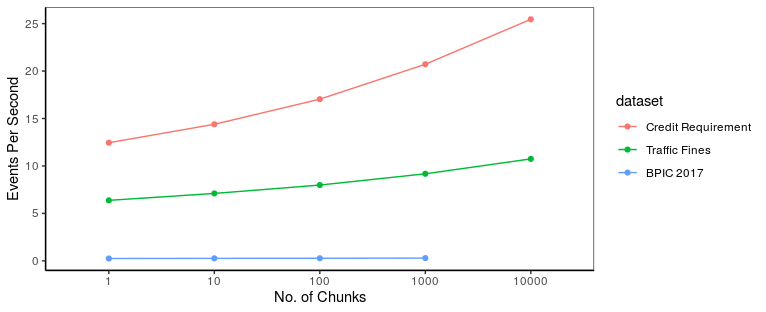
\includegraphics[width=.95\columnwidth]{figures/throughput.png}
	\caption{Throughput Benchmark: Events per Second vs no. of Chunks.}
	\label{fig:throughput}
\end{figure}

\textbf{Throughput Benchmark.} In fig~\ref{fig:throughput}, we report the number of events per second for different number of chunks. We can observe that, for datasets with smaller average number of events per trace, as in the Traffic Fines log, the throughput increase largely with increasing the number of chunks. However, increasing the average number of events per trace, as in both Credit Requirement log and BPIC 2017 log, makes the throughput grows slower. The reason for that is with the larger average of events per trace, the size of the data grows rapidly because of padding. We choose padding to avoid revealing the number of events per each trace.
%\begin{figure}[!htb]
%	\centering
%\subfloat[Data Sent]{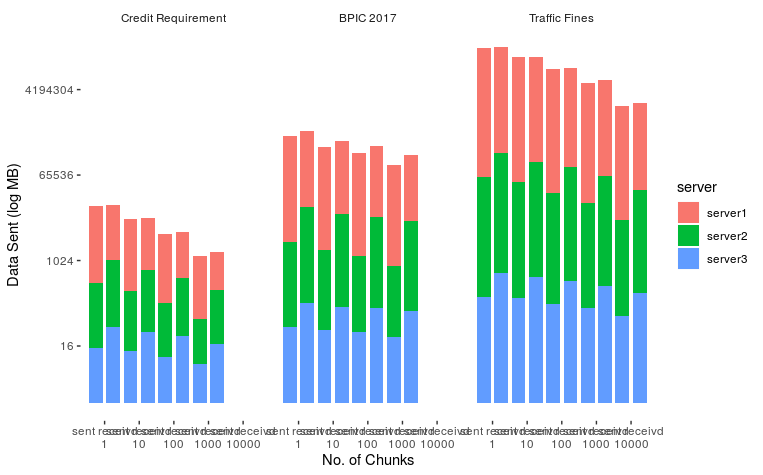
\includegraphics[width=0.5\textwidth, keepaspectratio]{figures/communication.png}\label{fig:comm_sent}}
%\subfloat[Data Received]{\includegraphics[width=0.5\textwidth, keepaspectratio]{figures/communication_received.png}\label{fig:comm_reveived}}

%\caption[]{Data Sent and Received for different servers vs the number of Chunks.}
%\label{fig:comm}
%\end{figure}

\begin{figure}[!htb]
	\centering
	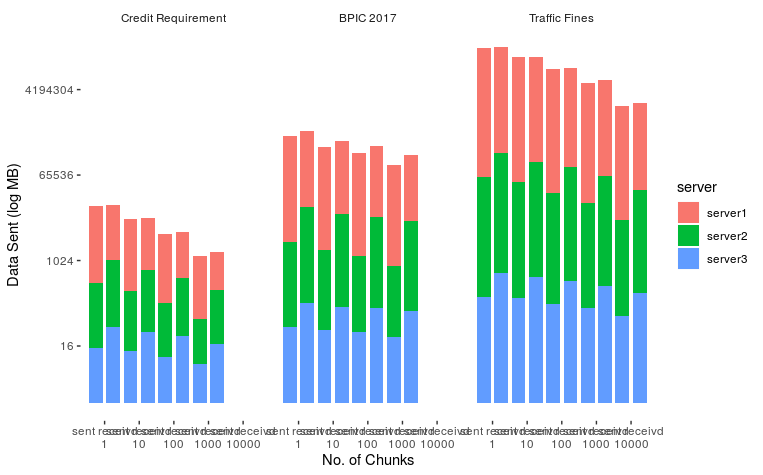
\includegraphics[width=.95\columnwidth]{figures/communication.png}
	\caption{Communication Benchmark: Data Sent and Received vs no. of Chunks.}
	\label{fig:comm}
\end{figure}

\textbf{Communication Overhead Benchmark.} In fig~\ref{fig:comm} , we present the amount of data sent and received at each server. We can observe that the communication overhead decreases with increasing the number of chunks. There are differences between the values reported for the different servers, because our implementation inside Sharemind uses asymmetry of comparison protocols.

Also, we can observe from fig~\ref{fig:comm} that the communication overhead increases with increasing the number of unique events per event log. That happens as the outer product for larger matrix size costs more communications. 

